
\testsection{Default options log plot}
\testsubsection{Default size}
\begin{tikzpicture}
\begin{loglogaxis}
\loglogtestplot
\end{loglogaxis}
\end{tikzpicture}

\testsubsection{Small size}
\begin{tikzpicture}
\begin{loglogaxis}[width=6cm]
\loglogtestplot
\end{loglogaxis}
\end{tikzpicture}
%
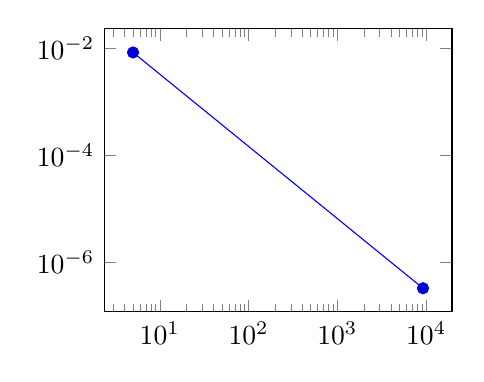
\begin{tikzpicture}
\begin{loglogaxis}[width=6cm]
\addplot plot coordinates {
	(5,	8.311600e-03)
	(9217,	3.261015e-07)
};
\end{loglogaxis}
\end{tikzpicture}

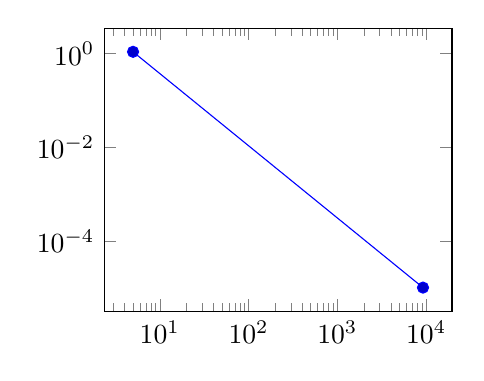
\begin{tikzpicture}
\begin{loglogaxis}[width=6cm,ytick={1.0e0,1e-2,1e-4}]
\addplot plot coordinates {
	(5,	1.1e-00)
	(9217,	1e-05)
};
\end{loglogaxis}
\end{tikzpicture}

\testsubsection{Very small size}
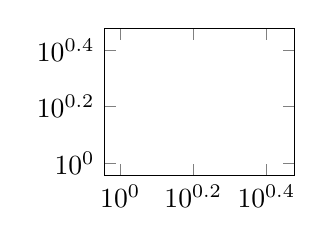
\begin{tikzpicture}
\begin{loglogaxis}[width=4cm]
\loglogtestplot
\end{loglogaxis}
\end{tikzpicture}

\testsubsection{Large size}
\begin{tikzpicture}
\begin{loglogaxis}[width=\textwidth]
\loglogtestplot
\end{loglogaxis}
\end{tikzpicture}

\testsubsection{Large size; large range}
\begin{tikzpicture}
\begin{loglogaxis}[width=\textwidth]
\addplot coordinates {
	(1e0,1e12)
	(1e16,1e-12)
};
\end{loglogaxis}
\end{tikzpicture}


\testsubsection{Extremely small y range for log plot} 
\testsubsubsection{Without extra ticks, enlargelimits=false}
\begin{tikzpicture}
\begin{loglogaxis}[
	enlargelimits=false,
]
\addplot coordinates {
	(1e0,1.5e-4)
	(1e24,2e-3)
};
\end{loglogaxis}
\end{tikzpicture}

\testsubsubsection{With extra ticks, enlargelimits=false}
extra y ticks=\{2e-4,3e-4,4e-4,5e-4,6e-4,7e-4,8e-4,9e-4,1.2e-3\}

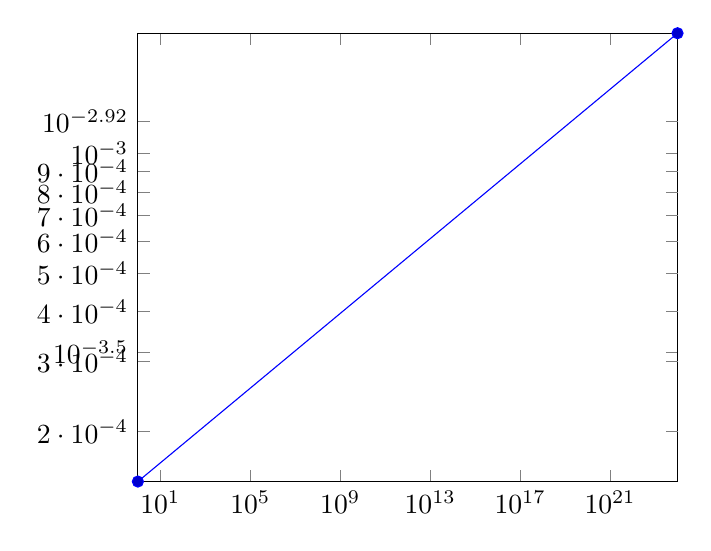
\begin{tikzpicture}
\begin{loglogaxis}[
	enlargelimits=false,
	extra y ticks={2e-4,3e-4,4e-4,5e-4,6e-4,7e-4,8e-4,9e-4,1.2e-3},
]
\addplot coordinates {
	(1e0,1.5e-4)
	(1e24,2e-3)
};
\end{loglogaxis}
\end{tikzpicture}

\testsection{Semilogy plot}
\begin{tikzpicture}
	\begin{semilogyaxis}[xlabel=Index,ylabel=Value]
	\addplot[color=blue,mark=*] plot coordinates {
		(1,8)
		(2,16)
		(3,32)
		(4,64)
		(5,128)
		(6,256)
		(7,512)
	};
	\end{semilogyaxis}
\end{tikzpicture}

\testsection{Semilogx plot}
\begin{tikzpicture}
	\begin{semilogxaxis}[xlabel=Index,ylabel=Value]
	\addplot[color=blue,mark=*] plot coordinates {
		(8,1)
		(16,2)
		(32,3)
		(64,4)
		(128,5)
		(256,6)
		(512,7)
	};
	\end{semilogxaxis}
\end{tikzpicture}

\testsubsection{Extra ticks}
Options:

extra x ticks=\{6e0,9e0,2e1,3e1,4e1,5e2,6e2,7e2,8e2,9e2\},

extra x tick style=\{/pgf/number format/sci subscript,font=footnotesize\},

\begin{tikzpicture}
	\begin{semilogxaxis}[xlabel=Index,ylabel=Value,
		width=\textwidth,
		extra x ticks={6e0,9e0,2e1,3e1,4e1,5e2,6e2,7e2,8e2,9e2},
		extra x tick style={/pgf/number format/sci subscript,font=\footnotesize},
	]
	\addplot[color=blue,mark=*] plot coordinates {
		(8,1)
		(16,2)
		(32,3)
		(64,4)
		(128,5)
		(256,6)
		(512,7)
	};
	\end{semilogxaxis}
\end{tikzpicture}
